\documentclass[dvipdfmx, twocolumn]{jsarticle}

\usepackage[version=3]{mhchem}
\usepackage{amsmath}
\usepackage[siunitx]{circuitikz}
\usepackage{graphicx}
\usepackage{here}

\setlength\parindent{0pt}

\begin{document}
\title{A2実験総合レポート}
\author{03190449  堀 紡希}
\date{\ 6月11日}
\maketitle
\section{実験目的}

現在コンピュータを扱う上ではデジタル回路が重要だが、応用的な難しい回路ではよりシンプルなアナログ回路が活躍する場合もあるので、まずはアナログ回路の基本を学習する。
\section{実験原理}
発振

増幅器の出力の一部が入力側に戻ることを帰還といい、入力に加算されることを正帰還、減算されることを負帰還という。
特に実験テキスト図A2.7の負帰還回路では増幅器で反転された$v_{i}$が減算されているので結果として正帰還になる。$v_{i}$が$A\beta$倍されて加えられる過程がループして増幅されていく。
$A, \beta$は周波数により変化するので、増幅率$A_{v} = \frac{A}{1+A\beta}$の分母が0になる周波数、すなわち$A\beta = -1$となる周波数が存在すればその周波数の信号の振幅は雑音のような小さな信号であっても無限大に増幅される。これを発振という。

\section{実験方法}

National Instruments社の設計/プロトタイプ環境システムNI ELVISのプロトタイプボード上に回路を組んで実験を行なった。
\begin{enumerate}
\item[1日目]

\begin{itemize}
\item まず班員でNI ELVISの操作とブレッドボードの扱いに習熟した。

\item 次に実験テキスト図A2.24に示されている回路を用いて、出力電圧がなるべく小さくなるように可変抵抗の値を調整してオペアンプのオフセット調整を行なった。

\item オフセット調整を行なった回路を使って実験テキスト図A2.25の反転増幅回路を$R_{1}=9.94$ k$\Omega, R_{2} = 98.7$k$\Omega$を用いてゲインを約20dB、$R_{1}=0.997$ k$\Omega, R_{2} = 98.7$ k$\Omega$としてゲインを約40dBとしてそれぞれ構成しボーデ線図をBodeモードを用いて測定しいくつかの周波数の正弦波を入力した時の波形をFGENとScopeモードを用いて観測した。

\item また、同じように$R_{1}=9.94$ k$\Omega, R_{2} = 98.7$ k$\Omega$、$R_{1}=0.997$ k$\Omega, R_{2} = 98.7$ k$\Omega$として実験テキスト図A2.11の非反転増幅回路をゲインを20dB,40dBとしてボーデ線図、出力波形を観測した。

\item 次に実験テキスト図A2.14の微分回路を構成した。素子の値は$R_{f} = 98.5$ k$\Omega$, $R_{r} = 0.997$ k$\Omega$, $C_{r} = 0.443\mu$ F, $C_{f} = 0.59$ nFとした。これもまたこれまでと同様にボーデ線図を測定した。ただし、$R_{r}, C_{f}$ありの回路と$C_{f}$なしと$R_{r}$なしと$R_{r}, C_{f}$なしの四つの回路で測定した。また$R_{r}, C_{f}$ありの回路について、微分動作、反転増幅、積分動作をするそれぞれの周波数領域の方形波応答を測定した。
\end{itemize}

\item[2日目]
\begin{itemize}

\item 実験テキスト図A2.16に示されているウィーンブリッジ回路を可変抵抗の$R = 9.89$k$\Omega$, 帰還部の$R = 9.93$k$\Omega$, $R_{r} = 0.991$k$\Omega$, $R_{f} = 5.12$k$\Omega$, 並列部のキャパシタ$C_{1} = 9.94$nF, 直列部のキャパシタ$C_{2} = 9.90$nFとして構成し、可変抵抗を調整して入力を入れなくても発振するように調整した。
\item 可変抵抗をそのままにして、オシロスコープで出力波形、スペクトルアナライザで周波数スペクトルの変化を観測した

\item 可変抵抗の値をピークと違うものにしていくつか出力波形と周波数スペクトルを観測した。

\item 実験テキスト図A2.17のようにしてX点の電圧を測定し開ループ利得の周波数特性を測定した。これもいくつかの可変抵抗の値で測定した。

\end{itemize}

\item[3日目]

\begin{itemize}

\item 遮断周波数f = 1kHz, $\epsilon = 1.0$としてP3実験で設計したButterworthとChebyshevの低域通過フィルタを図P3.6のように構成し周波数特性とステップ応答を測定した。

Butterworthで$L_{1} = 3\mu$H(内部抵抗$15.5\Omega$), $L_{2} = 1\mu$H(内部抵抗$5.4\Omega$), C = 50.5$\mu$F, I = $4.2\Omega$, Chebyshevで$L_{1} = 12\mu$H(内部抵抗$70.2\Omega$), $L_{2} = 10\mu$H(内部抵抗$61.5\Omega$), C = 4.02$\mu$F, I = $52.9\Omega$とした。

\item 同様に遮断周波数f = 1kHzとしてP3実験で設計したButterworthとChebyshevの高域通過フィルタを図P3.6のように構成し周波数特性とステップ応答を測定した。

Butterworthで$C_{1} = 11.1\mu$F, $C_{2} = 39.7\mu$F, L = 1$\mu$H(内部抵抗$5.0\Omega$), I = $8.3\Omega$, Chebyshevで$C_{1} = 11.1\mu$F, $C_{2} = 11.03\mu$F, L = $1\mu$H(内部抵抗$5.0\Omega$), I = $7.3\Omega$とした。


\end{itemize}

\item[4日目]
\begin{itemize}

\item 実験テキスト図A2.21に示されている低域通過型アクティブフィルタを構成し、周波数応答と方形波(1Hz)応答を観測した。$V_{in}$の方の抵抗$R_{1} = 1.125$k$\Omega$, $R_{2} = 1.123$k$\Omega$, $C = 0.1131\mu$F, $2C = 0.252\mu$Fとした。

\item 実験テキスト図A2.22に示されている高域通過型アクティブフィルタを構成し、周波数応答と方形波(1Hz)応答を観測した。$R = 1.125$k$\Omega$, 入力側のキャパシタ$C_{1} = 0.986\mu$F, $C_{2} = 0.893\mu$F, $2R = 2.274$k$\Omega$とした。

\end{itemize}
\end{enumerate}
\section{実験結果}
\begin{enumerate}

\item[1日目]
\begin{itemize}

\item オフセット調整

非常に抵抗の変化に対してオフセットの変化が敏感であったため、オフセットを0Vにすることが理想ではあるが難しかったため+50mVくらいになるまで調整をした。


\item 反転増幅回路
20dBの設計の時、周波数特性は図1, 2のようになった。増幅率の理論値は19.93dBで、位相は低周波のみ180度のズレになっており確かに反転されている。Bodeモードの仕様上周波数が158kHzまでしか取れていないが、高周波の領域におけるグラフの傾きは-16.5dB/decになっており理論値-20dB/decより17\%ほど小さくなっている。


\begin{figure}[H]
\begin{center}
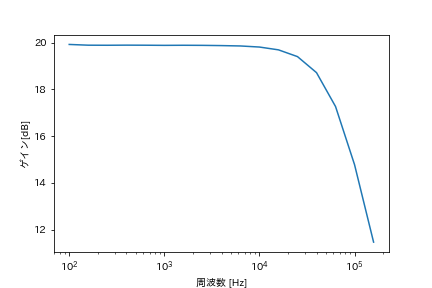
\includegraphics[scale = 0.5]{G20dB.png}
\caption{ゲイン20dBの反転増幅回路の振幅特性}
\end{center}
\end{figure}

\begin{figure}[H]
\begin{center}
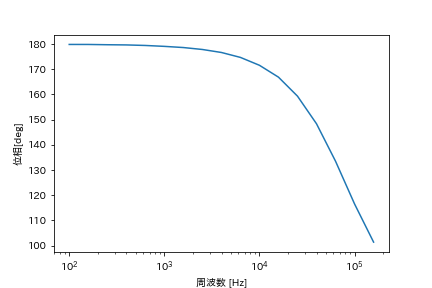
\includegraphics[scale = 0.5]{P20dB.png}
\caption{ゲイン20dBの反転増幅回路の位相特性}
\end{center}
\end{figure}


次に40dBの設計の時の測定結果が図3, 4である。位相特性は20dBの時と同じであるが振幅特性は傾きが-19.97と理論値と1\%以下の誤差となった。
低周波では増幅率が38.563と3\%ほどの誤差となっている。


\begin{figure}[H]
\begin{center}
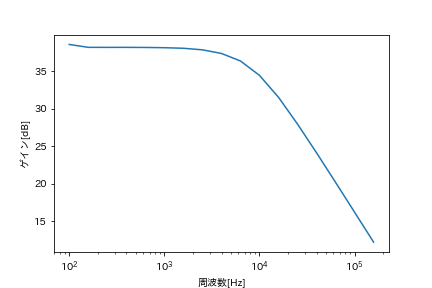
\includegraphics[scale = 0.5]{G40dB.png}
\caption{ゲイン40dBの反転増幅回路の振幅特性}
\end{center}
\end{figure}

\begin{figure}[H]
\begin{center}
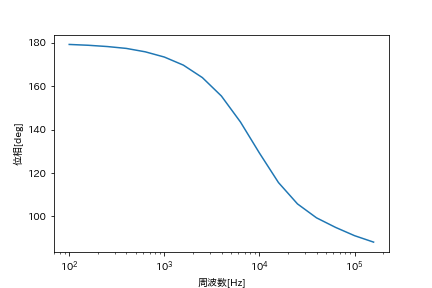
\includegraphics[scale = 0.5]{P40dB.png}
\caption{ゲイン40dBの反転増幅回路の位相特性}
\end{center}
\end{figure}

図5はオシロスコープで測定した20dB反転増幅回路の応答波形である。入力波形は1kHzの正弦波。確かに位相が逆転し、入力波形のピークが0.0264V,出力波形が0.268Vとなっているからおよそ10倍になっており確かに20dB増幅している。
\begin{figure}[H]
\begin{center}
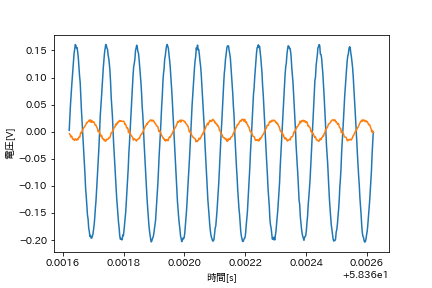
\includegraphics[scale = 0.5]{wave20dB.png}
\caption{ゲイン20dBの反転増幅回路の応答波形}
\end{center}
\end{figure}

\item 非反転増幅回路

20dBの設計の時、周波数特性は図6, 7のようになった。40dBの場合は図8, 9に示した。増幅率の理論値は20.8dB。位相は低周波のみ0度のズレになっており確かに反転されていない。振幅特性の傾きは-1.3ほどと、とても小さかった。これはこの測定範囲の周波数が低かったためで、落ちきる前であったためと考えられる。確かに位相も図8に比べると落ち方が小さくなっている。


\begin{figure}[H]
\begin{center}
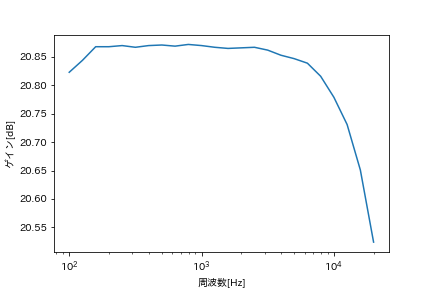
\includegraphics[scale = 0.5]{nG20dB.png}
\caption{ゲイン20dBの非反転増幅回路の振幅特性}
\end{center}
\end{figure}

\begin{figure}[H]
\begin{center}
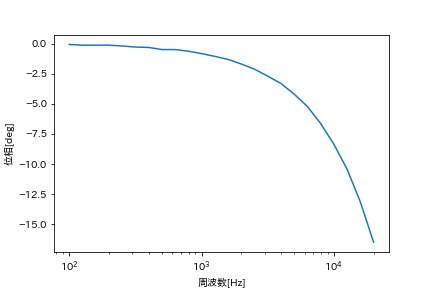
\includegraphics[scale = 0.5]{nP20dB.png}
\caption{ゲイン20dBの非反転増幅回路の位相特性}
\end{center}
\end{figure}


40dBの場合ゲインの理論値は40.0で3.5\%ほどの誤差がある。

\begin{figure}[H]
\begin{center}
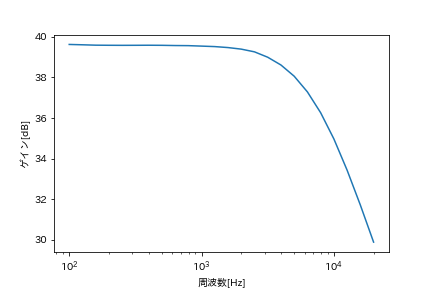
\includegraphics[scale = 0.5]{nG40dB.png}
\caption{ゲイン40dBの非反転増幅回路の振幅特性}
\end{center}
\end{figure}

\begin{figure}[H]
\begin{center}
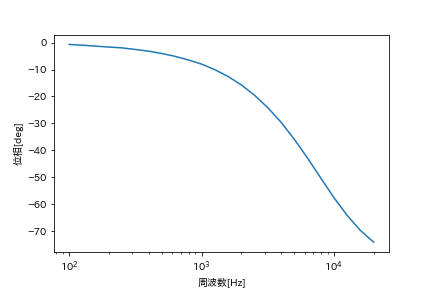
\includegraphics[scale = 0.5]{nP40dB.png}
\caption{ゲイン40dBの非反転増幅回路の位相特性}
\end{center}
\end{figure}


図10はオシロスコープで測定した20dB非反転増幅回路の応答波形である。こちらも入力波形は1kHzの正弦波である。図5と見比べるとよくわかるが確かに位相を反転させずに増幅している。

\begin{figure}[H]
\begin{center}
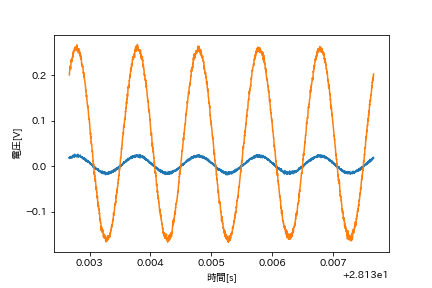
\includegraphics[scale = 0.5]{waven20dB.png}
\caption{ゲイン20dBの非反転増幅回路の応答波形}
\end{center}
\end{figure}


\item 微分回路


図11, 12は微分回路のボーデ線図である。200Hzくらいまでは位相が90度遅れる微分回路としてはたらき、5kHzくらいまでは位相が180度遅れで増幅率が15dBほどの反転増幅回路、それより上では270度遅れ(90度進み)の積分回路としてはたらいている。
\begin{figure}[H]
\begin{center}
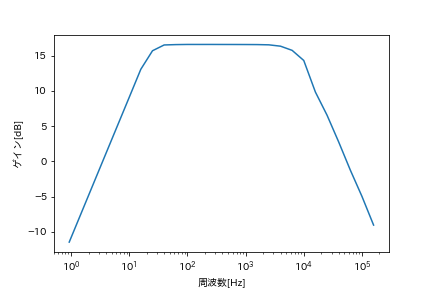
\includegraphics[scale = 0.5]{dGRrCf.png}
\caption{微分回路の振幅特性}
\end{center}
\end{figure}

\begin{figure}[H]
\begin{center}
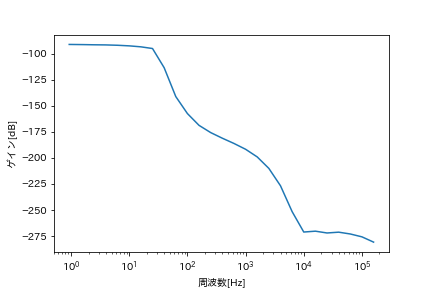
\includegraphics[scale = 0.5]{dPRrCf.png}
\caption{微分回路の位相特性}
\end{center}
\end{figure}


図13,14は $R_{r}$を取り去った微分回路のボーデ線図である。図11,12に比べて微分回路としてはたらく周波数が広くなっている。また、ピークの増幅率は40dBほどと大きくなっている。
\begin{figure}[H]
\begin{center}
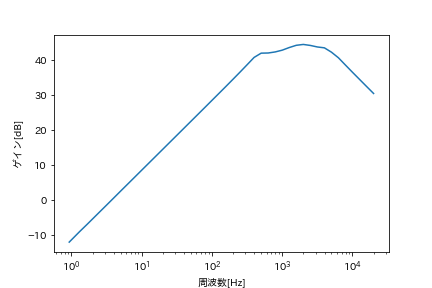
\includegraphics[scale = 0.5]{dGCf.png}
\caption{微分回路($R_{r}なし$)の振幅特性}
\end{center}
\end{figure}

\begin{figure}[H]
\begin{center}
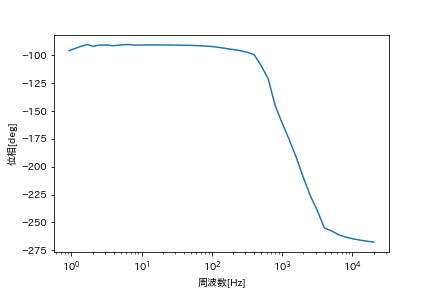
\includegraphics[scale = 0.5]{dPCf.png}
\caption{微分回路($R_{r}なし$)の位相特性}
\end{center}
\end{figure}


図15,16は $C_{f}$を取り去った微分回路のボーデ線図である。図11,12に比べて反転増幅回路としてはたらく領域が10kHzあたりのところまで広くなっている。また、位相特性が滑らかになっている。

\begin{figure}[H]
\begin{center}
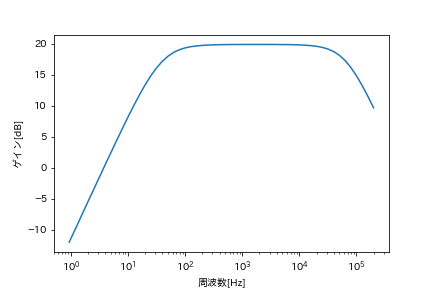
\includegraphics[scale = 0.5]{dGRr.png}
\caption{微分回路($C_{f}なし$)の振幅特性}
\end{center}
\end{figure}

\begin{figure}[H]
\begin{center}
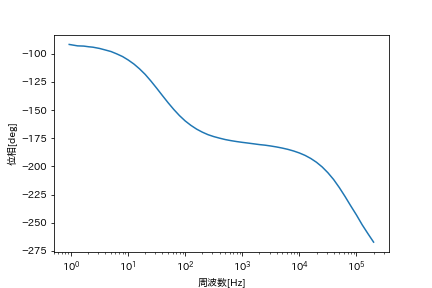
\includegraphics[scale = 0.5]{dPRr.png}
\caption{微分回路($C_{f}なし$)の位相特性}
\end{center}
\end{figure}

図17,18は $R_{r}, C_{f}$を取り去った微分回路のボーデ線図である。増幅率が0dBになっており他のグラフと全く形が違うので回路を組み間違えるなどして妥当な結果が得られなかったと考えられる。
\begin{figure}[H]
\begin{center}
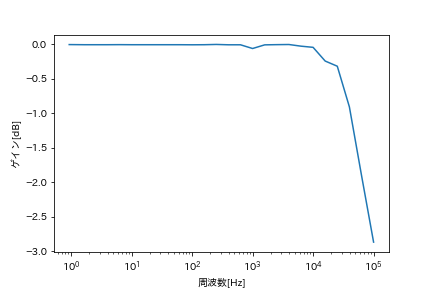
\includegraphics[scale = 0.5]{dG.png}
\caption{微分回路($R_{r}, C_{f}なし$)の振幅特性}
\end{center}
\end{figure}

\begin{figure}[H]
\begin{center}
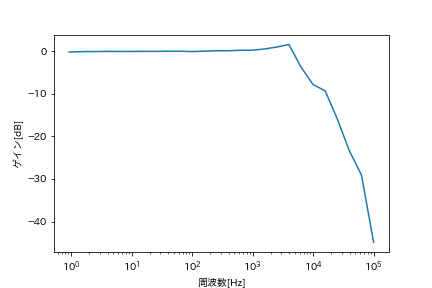
\includegraphics[scale = 0.5]{dP.png}
\caption{微分回路($R_{r}, C_{f}なし$)の位相特性}
\end{center}
\end{figure}

図19は微分回路の方形波(10Hz)に対するステップ応答である。低周波であるため微分回路としてはたらき、確かにデルタ関数の列のようなものが得られている。
\begin{figure}[H]
\begin{center}
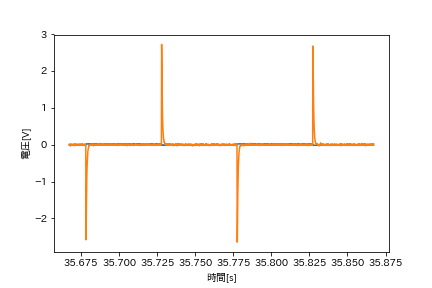
\includegraphics[scale = 0.5]{wavedlow.png}
\caption{微分回路のステップ応答(10Hz)}
\end{center}
\end{figure}

図20は微分回路の方形波(2kHz)に対するステップ応答である。やや歪んでいるが反転増幅回路としてはたらいていることが見て取れる。

\begin{figure}[H]
\begin{center}
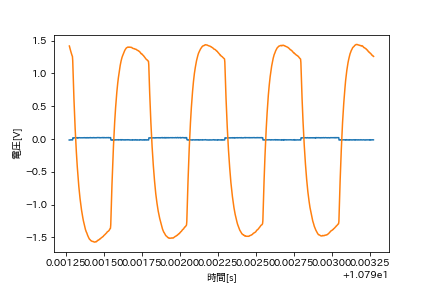
\includegraphics[scale = 0.5]{wavedmid.png}
\caption{微分回路のステップ応答(2kHz)}
\end{center}
\end{figure}


図21は微分回路の方形波(20kHz)に対するステップ応答である。一次関数(=定数関数の積分)が並んでいるような形になっており位相が反転しているが高周波では積分としての動作をしていることがわかる。

\begin{figure}[H]
\begin{center}
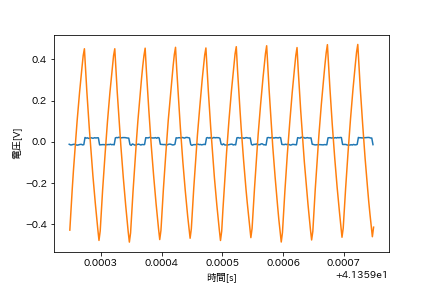
\includegraphics[scale = 0.5]{wavedhigh.png}
\caption{微分回路のステップ応答(20kHz)}
\end{center}
\end{figure}


\end{itemize}

\item[2日目]
\begin{itemize}
\item ウィーンブリッジ回路

可変抵抗を調整したところ、k = 0.517となるところで発振が起こった。

図22,23は発振した時とそうでない時のスペクトルの違いである。発振している時はスペクトルが最大20dBであるのに対して発振していない時は約-77dBという大変小さな値になっていた。
\begin{figure}[H]
\begin{center}
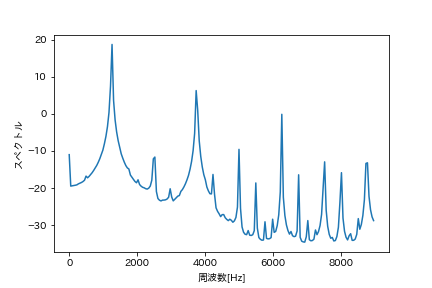
\includegraphics[scale = 0.5]{spha.png}
\caption{ウィーン発振回路の周波数スペクトル(発振時)}
\end{center}
\end{figure}

\begin{figure}[H]
\begin{center}
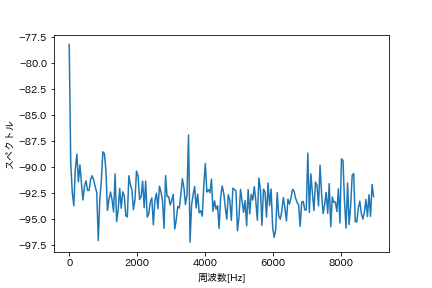
\includegraphics[scale = 0.5]{spnha.png}
\caption{ウィーン発振回路の周波数スペクトル(非発振時)}
\end{center}
\end{figure}




\end{itemize}
\item[3日目]
\begin{itemize}

\item LPF

以下が設計したLPFのボーデ線図である。Butterworthではややゲインが落ち込むのが早いがあとはChebyshevにリプルも現れており、概ね予想通りの結果が得られた。
\begin{figure}[H]
\begin{center}
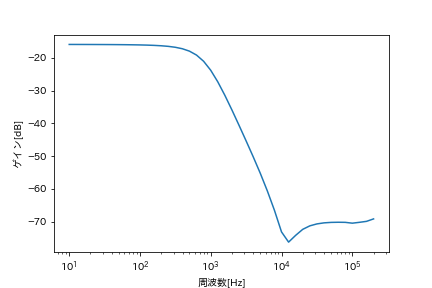
\includegraphics[scale = 0.5]{BGLPF.png}
\caption{Butterworth型LPFの振幅特性}
\end{center}
\end{figure}

\begin{figure}[H]
\begin{center}
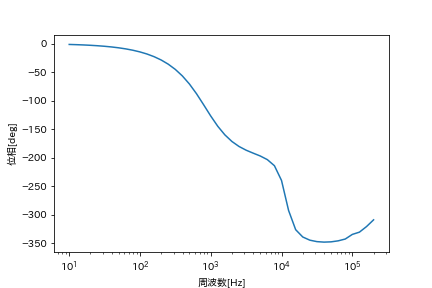
\includegraphics[scale = 0.5]{BPLPF.png}
\caption{Butterworth型LPFの位相特性}
\end{center}
\end{figure}

\begin{figure}[H]
\begin{center}
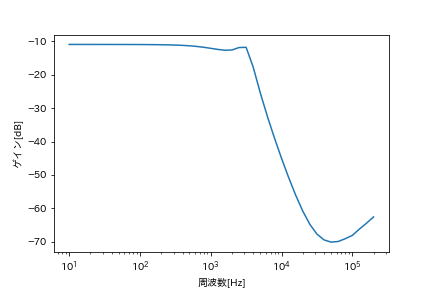
\includegraphics[scale = 0.5]{CGLPF.png}
\caption{Chebyshev型LPFの振幅特性}
\end{center}
\end{figure}

\begin{figure}[H]
\begin{center}
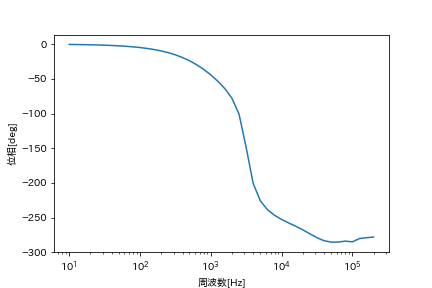
\includegraphics[scale = 0.5]{CPLPF.png}
\caption{Chebyshev型LPFの位相特性}
\end{center}
\end{figure}

\item HPF

以下が設計したHPFのボーデ線図である。Chebyshevの方が低周波の方で180度に近い位相差が現れるはずであったが大きくずれてしまっている。

\begin{figure}[H]
\begin{center}
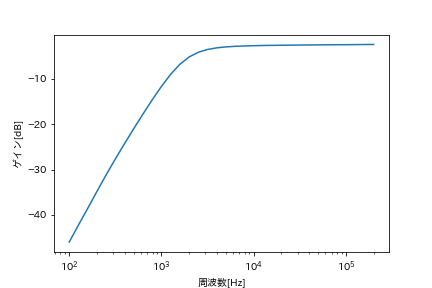
\includegraphics[scale = 0.5]{BGHPF.png}
\caption{Butterworth型HPFの振幅特性}
\end{center}
\end{figure}

\begin{figure}[H]
\begin{center}
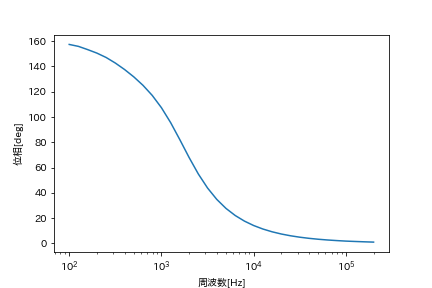
\includegraphics[scale = 0.5]{BPHPF.png}
\caption{Butterworth型HPFの位相特性}
\end{center}
\end{figure}

\begin{figure}[H]
\begin{center}
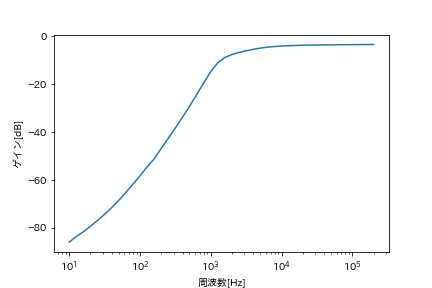
\includegraphics[scale = 0.5]{CGHPF.png}
\caption{Chebyshev型HPFの振幅特性}
\end{center}
\end{figure}

\begin{figure}[H]
\begin{center}
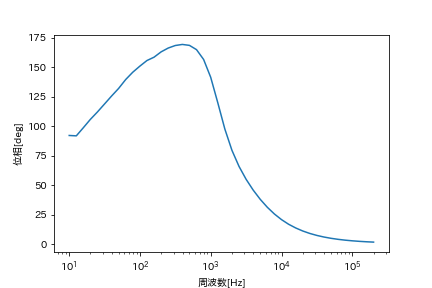
\includegraphics[scale = 0.5]{CPHPF.png}
\caption{Chebyshev型HPFの位相特性}
\end{center}
\end{figure}


以下の図がパッシブフィルタのステップ応答である。この波形がインパルス応答の積分、つまり、伝達関数の積分になると考えられる。


\begin{figure}[H]
\begin{center}
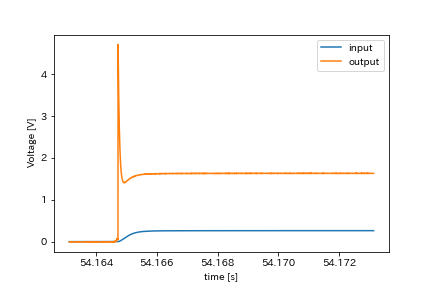
\includegraphics[scale = 0.5]{stepBL.png}
\caption{Butterworth型LPFのステップ応答}
\end{center}
\end{figure}


\begin{figure}[H]
\begin{center}
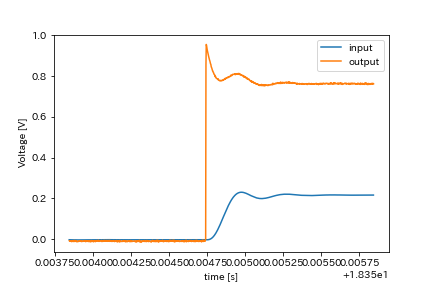
\includegraphics[scale = 0.5]{stepCL.png}
\caption{Chebyshev型LPFのステップ応答}
\end{center}
\end{figure}

LPFでは入力した方形波の大きさが違ったが、HPFでは同じだったので同じグラフにまとめた。
\begin{figure}[H]
\begin{center}
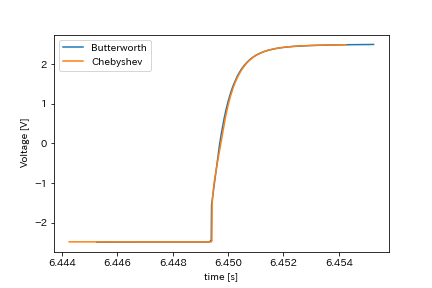
\includegraphics[scale = 0.5]{stepHPF.png}
\caption{HPFのステップ応答}
\end{center}
\end{figure}


\end{itemize}
\item[4日目]

\begin{itemize}


\item 低域通過型アクティブフィルタ

\begin{figure}[H]
\begin{center}
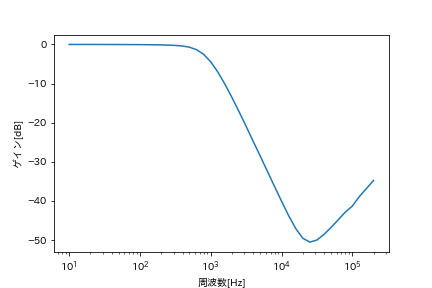
\includegraphics[scale = 0.5]{GactL.png}
\caption{アクティブLPFの振幅特性}
\end{center}
\end{figure}

\begin{figure}[H]
\begin{center}
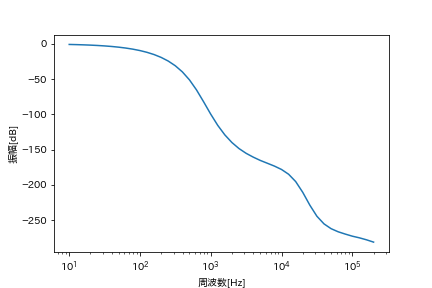
\includegraphics[scale = 0.5]{PactL.png}
\caption{アクティブLPFの位相特性}
\end{center}
\end{figure}

\begin{figure}[H]
\begin{center}
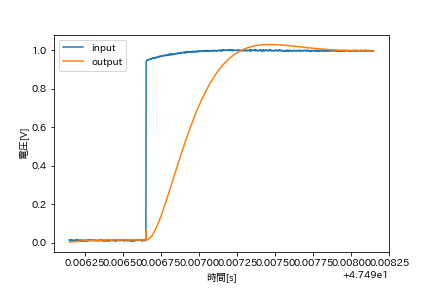
\includegraphics[scale = 0.5]{WactL.png}
\caption{アクティブLPFのステップ応答}
\end{center}
\end{figure}

\item 高域通過型アクティブフィルタ

\begin{figure}[H]
\begin{center}
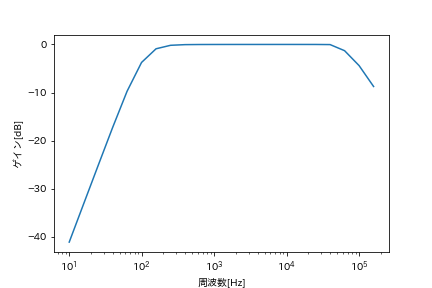
\includegraphics[scale = 0.5]{GactH.png}
\caption{アクティブHPFの振幅特性}
\end{center}
\end{figure}

\begin{figure}[H]
\begin{center}
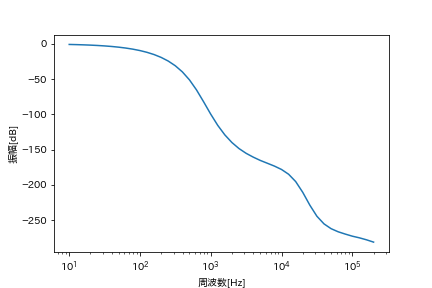
\includegraphics[scale = 0.5]{PactL.png}
\caption{アクティブHPFの位相特性}
\end{center}
\end{figure}

\begin{figure}[H]
\begin{center}
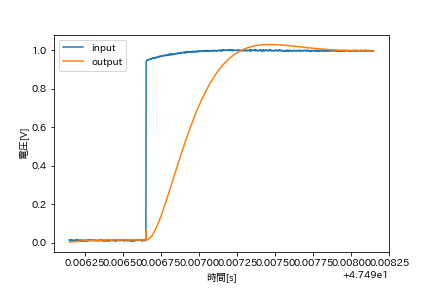
\includegraphics[scale = 0.5]{WactL.png}
\caption{アクティブHPFのステップ応答}
\end{center}
\end{figure}

\end{itemize}

\end{enumerate}

\section{考察課題}

\begin{enumerate}

\item[7.1(1)]
反転増幅回路、非反転増幅回路の遮断周波数

遮断周波数は反転増幅回路では20dBの回路で70kHz、40dBの回路で7kHz、非反転増幅回路では20dBの回路では読み取れず、40dBの回路では8kHzほどであった。

また遮断周波数を超えた領域での傾きは反転増幅回路で-16.5dB/dec(20dB), -20.0dB/dec(40dB), 非反転増幅回路で-18.3dB/dec(40dB)であった。

実験テキストの式A2.15より増幅率はおよそAに比例する。そして図A2.5よりAは-20dB/decで小さくなっていくので上で述べた反転増幅回路、非反転増幅回路の増幅率も同じように-20dB/dec程度の傾きで小さくなる。



\item[7.1(2)]
$R_{r}, C_{f}を付した微分回路の定性的性質$

図11, 12にその回路のボーデ線図が示してあるが、$f<f_{r} = 360$Hzで位相が90度遅れる、微分回路として働く。これは低周波においてキャパシタが高インピーダンスとなり$C_{r}$の働きが大きくなるからである。

$f_{r}<f<f_{f} \simeq 2700$Hzの時は位相が180度ずれており反転増幅回路として働いている。これは中域の周波数においてキャパシタが低インピーダンスとなり$R_{r}, R_{f}$の働きが大きくなるからである。

$f_{f}<f$の時は位相が270度遅れ(90度進み)ており積分回路として働いている。これは高い周波数においてキャパシタがさらに低インピーダンスとなり$R_{r}, C_{f}$の働きが大きくなるからである。

方形波応答は微分回路として働く領域ではステップ波が微分されデルタ関数列となっている(図19)。反転増幅回路として働く領域ではステップ波が位相を反転し増幅されている(図20)。高周波では定数関数が積分され、傾きが-1倍された一次関数の列になっており確かにそれぞれの性質を反映している(図21)。




\item[独自考察]ゲインの定量的考察

反転増幅回路は20dB, 40dBで設計したが、実際には素子の値が理想通りではないので少しずれている。20dBの時は$R_{1} = 9.94$k$\Omega$, $R_{2} = 98.7$k$\Omega$としたのでゲインの理論値は19.94dBとなり、実験値19.92dBに0.2\%ほど近づいた。

同様に40dBの時、理論値は39.912dBとなりこれも理論値に0.2\%ほど近づいた。しかし、素子の値を考慮してもまだ3\% ほどずれているが、これはブレッドボード等の測定系の内部抵抗、オペアンプの性能の問題が原因として考えられる。



\item[7.2(3)]
発振を開始するk

実験テキストの式A2.46
\[ A_{v}(s) = A\frac{(sCR)^{2}+3sCR+1}{(sCR)^{2}+(3-kA)sCR+1}\]
より、k = 3/A, $\omega CR = 1$のとき分母が0になり発振する。

kの理論値はAから求めると0.49であるが実験値は0.52であった。これは誤差約6\% であり、可変抵抗の調整が手動であったことや理論通りの値の素子が用意できなかったことによるずれであると考えられる。


\end{enumerate}
\section{参考文献}
[1]東京大学工学部:「電気電子情報第一(前期) 実験テキスト」, 2019.

[2]廣瀬明:「電気電子計測」, 数理工学社, 2003.

\end{document}